\ifx\PREAMBLE\undefined
\documentclass{article}
\usepackage[format = hang, font = bf]{caption}
\usepackage{graphicx}
\usepackage{array}
\usepackage{amsmath}
\usepackage{mathtools}
\usepackage{boxedminipage}
\usepackage{listings}
\usepackage{makecell}%diagonal line in table
\usepackage{float}%allowing forceful figure[H]
\usepackage{xcolor}
\usepackage{amsfonts}%allowing \mathbb{R}
\usepackage{alltt}
\usepackage{url}
\def\UrlBreaks{\do\A\do\B\do\C\do\D\do\E\do\F\do\G\do\H\do\I\do\J\do\K\do\L\do\M\do\N\do\O\do\P\do\Q\do\R\do\S\do\T\do\U\do\V\do\W\do\X\do\Y\do\Z\do\[\do\\\do\]\do\^\do\_\do\`\do\a\do\b\do\c\do\d\do\e\do\f\do\g\do\h\do\i\do\j\do\k\do\l\do\m\do\n\do\o\do\p\do\q\do\r\do\s\do\t\do\u\do\v\do\w\do\x\do\y\do\z\do\0\do\1\do\2\do\3\do\4\do\5\do\6\do\7\do\8\do\9\do\.\do\@\do\\\do\/\do\!\do\_\do\|\do\;\do\>\do\]\do\)\do\,\do\?\do\'\do+\do\=\do\#\do\-}
\usepackage[breaklinks = true]{hyperref}
\lstset{language = matlab, breaklines = true, tabsize = 2, numbers = left, extendedchars = false, basicstyle = {\ttfamily \footnotesize}, keywordstyle=\color{blue!70}, commentstyle=\color{red!70}, frame=shadowbox, rulesepcolor=\color{red!20!green!20!blue!20}, numberstyle={\color[RGB]{0,192,192}}}

\begin{document}
\fi
\section{Neural network}
\subsection{Introduction}
Linear regression and logistic regression may not be pratical solutions to some machine learning problems because we will end up with too many features to deal with. As an example, suppose we want to conduct a logistic regression on a 100$\times$100 grey scale image (maybe trying to tell if it is an image of a car). If we want to take the quardatic items ($x_ix_j$) as features, there will be roughly $5\times10^7$ different features. If higher order items were to be taken into account, which is not uncommon, the number could become even higher. Trying to solve such problem with linear/logistic regression is obviously a dead end. The method to turn to in such case is neural network, which is the state-of-the-art technique for many machine learning applications.

Neural network dates back to a few decades ago when people started to try to mimic the way human brain works with computer. Due to the high requirement of computing capacity, it did not get into the spotlight until recent years. In a human neural cell, an electricity signal is inputted into the cell through an input wire called ``dendrite''. The cell processes the signal, and then sends a new signal out via an output wire called ``axon''. In machine learning, a logistic unit inside a neural network works in similar way. Different signals $x_i$ is inputted into the unit, and the unit outputs a new signal
\begin{equation} 
h_{\theta}(x) = \frac{1}{1+e^{-\theta^{\mathsf T}x}}
\end{equation}
as illustrated in Figure \ref{neuralunit}.
\begin{figure}[ht]
\centering
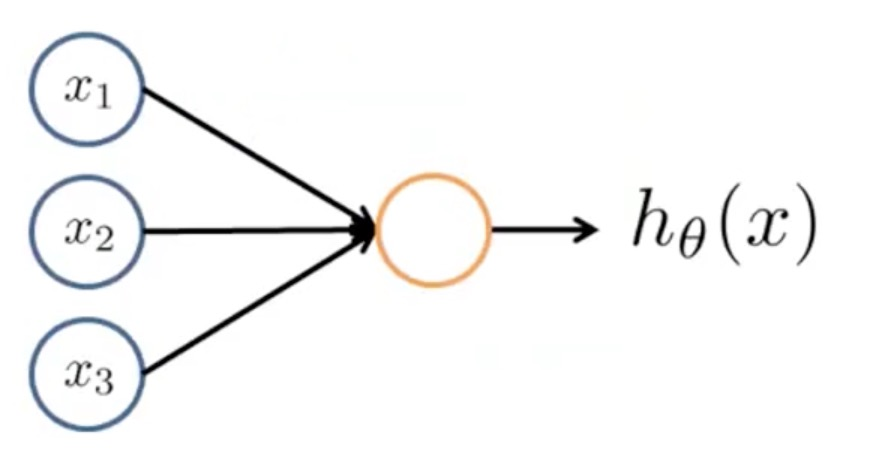
\includegraphics[width =0.6 \textwidth]{neuralunit.jpg}
\caption{Basic logistic unit in a neural network}\label{neuralunit}
\end{figure}

When a series of such logistic units, or neurons get connected, they form a neural network, as illustrated by Figure 
\ref{neuralnetwork}.

\begin{figure}[ht]
\centering
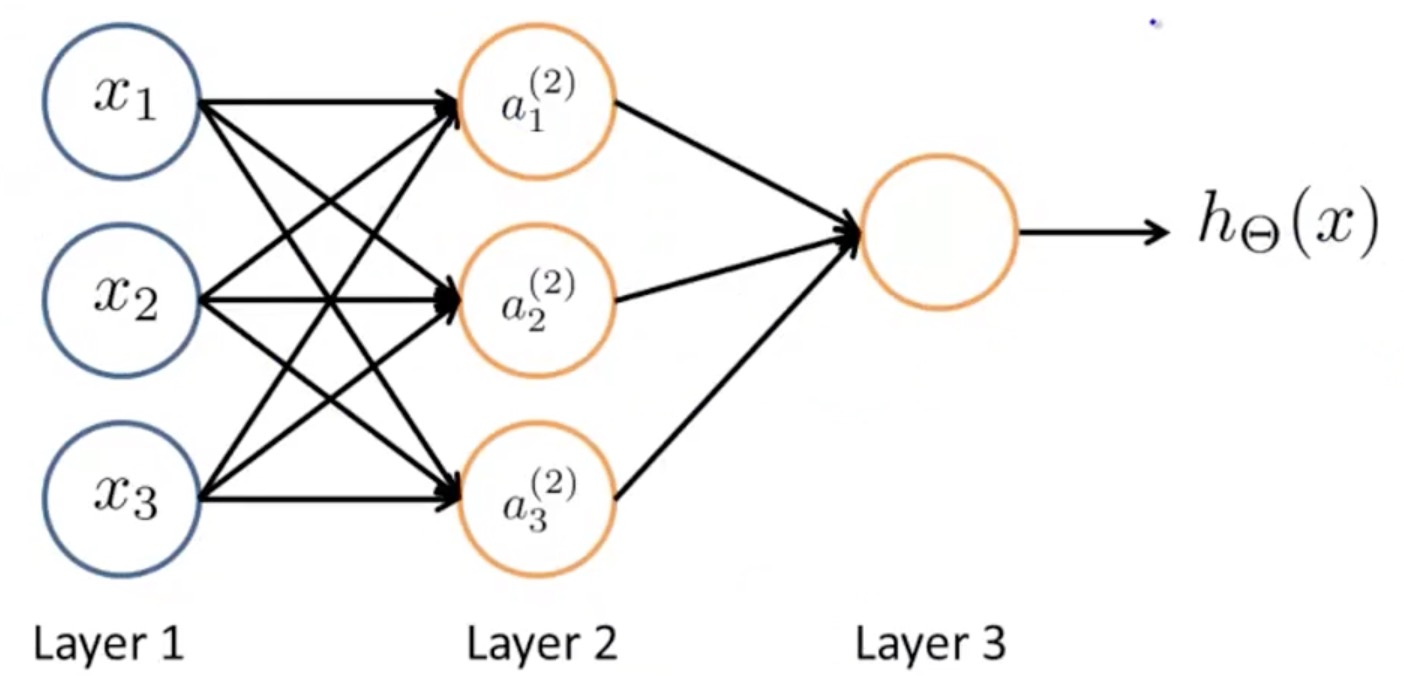
\includegraphics[width =0.8 \textwidth]{neuralnetwork.jpg}
\caption{A simple neural network}\label{neuralnetwork}
\end{figure}

Quantatively, by denoting the ``activation'' of unit $i$ in layer $j$ as $a_i^{(j)}$, the matrix of weights controlling function mapping from layer  $j$ to layer $j+1$ as $\Theta^{(j)}$, we have
\begin{equation}
\begin{split}\label{neuralnetworkeqs}
a_1^{(2)} &= g\left(\Theta^{(1)}_{10}x_0 + \Theta^{(1)}_{11}x_1 + \Theta^{(1)}_{12}x_2 + \Theta^{(1)}_{13}x_3\right)\\
a_2^{(2)} &= g\left(\Theta^{(1)}_{20}x_0 + \Theta^{(1)}_{21}x_1 + \Theta^{(1)}_{22}x_2 + \Theta^{(1)}_{23}x_3\right)\\
a_3^{(2)} &= g\left(\Theta^{(1)}_{30}x_0 + \Theta^{(1)}_{31}x_1 + \Theta^{(1)}_{32}x_2 + \Theta^{(1)}_{33}x_3\right)\\
h_{\theta}(x) &= a_1^{(3)} = g\left(\Theta^{(2)}_{10}a_0^{(2)} + \Theta^{(2)}_{11}a_1^{(2)} + \Theta^{(2)}_{12}a_2^{(2)} + \Theta^{(2)}_{13}a_3^{(2)}\right)
\end{split}
\end{equation}
in which $g(z)$ is the sigmoid function. The vectorized version of \eqref{neuralnetworkeqs} can be written as 
\begin{equation}
a^{(j+1)} = g\left(\Theta^{(j)}
\begin{bmatrix}
1\\
a^{(j)}
\end{bmatrix}
\right)
\end{equation}
If layer $j$ has $s_j$ neurons (not including the bias neuron $a_0^{(j)}=1$), it is clear that $\Theta^{(j)}$ is a 
$s_{j+1} * (s_j + 1)$ matrix.
\subsection{Examples}
\begin{figure}[ht]
\centering
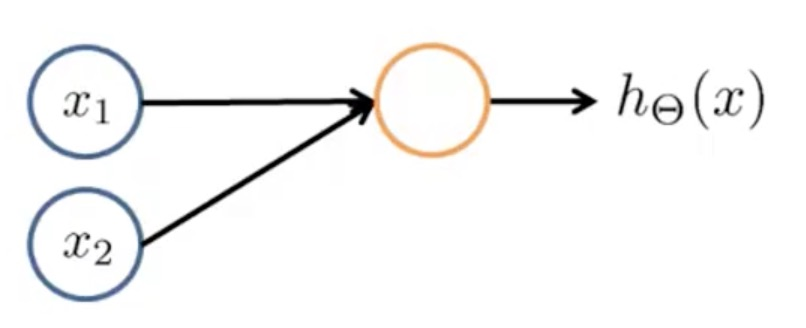
\includegraphics[width = 0.5 \textwidth]{neuraland.jpg}
\caption{Implementation of logical AND/OR with neural network}\label{neuraland}
\end{figure}
If we choose 
\begin{math}
\Theta^{(1)} = \begin{bmatrix}-30 & 20 & 20\end{bmatrix}
\end{math}
, it can be verified easily that the output will be $x_1$ AND $x_2$. Similarly, with
\begin{math}
\Theta^{(1)} = \begin{bmatrix}-10 & 20 & 20\end{bmatrix}
\end{math}
, the output will be $x_1$ OR $x_2$.

With the neural network shown in Figure \ref{neuralnot}, we can calculate NOT $x_1$ with 
\begin{math}
\Theta^{(1)} = \begin{bmatrix}10 & -20\end{bmatrix}
\end{math}
\begin{figure}[ht]
\centering
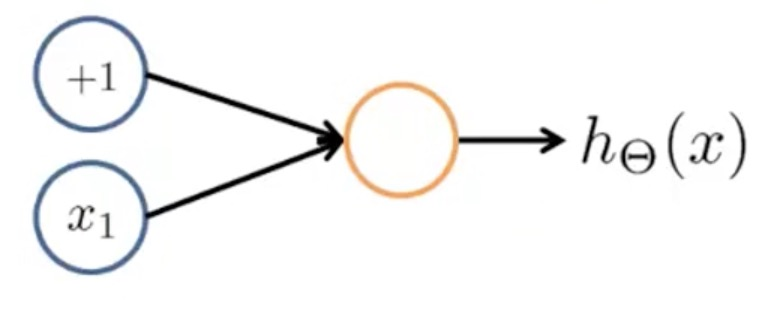
\includegraphics[width = 0.5 \textwidth]{neuralnot.jpg}
\caption{Implementation of logical NOT with neural network}\label{neuralnot}
\end{figure}

With the examples given above, we can calculate a more complex logical function XNOR. Note that
$$ x_1 \text{ XNOR } x_2 = (x_1 \text{ AND } x_2) \text{ OR } (NOT(x_1) \text{ AND } NOT(x_2))$$
Thus we can calculate XNOR with the neural network shown in Figure \ref{neuralxnor}.
\begin{figure}[ht]
\centering
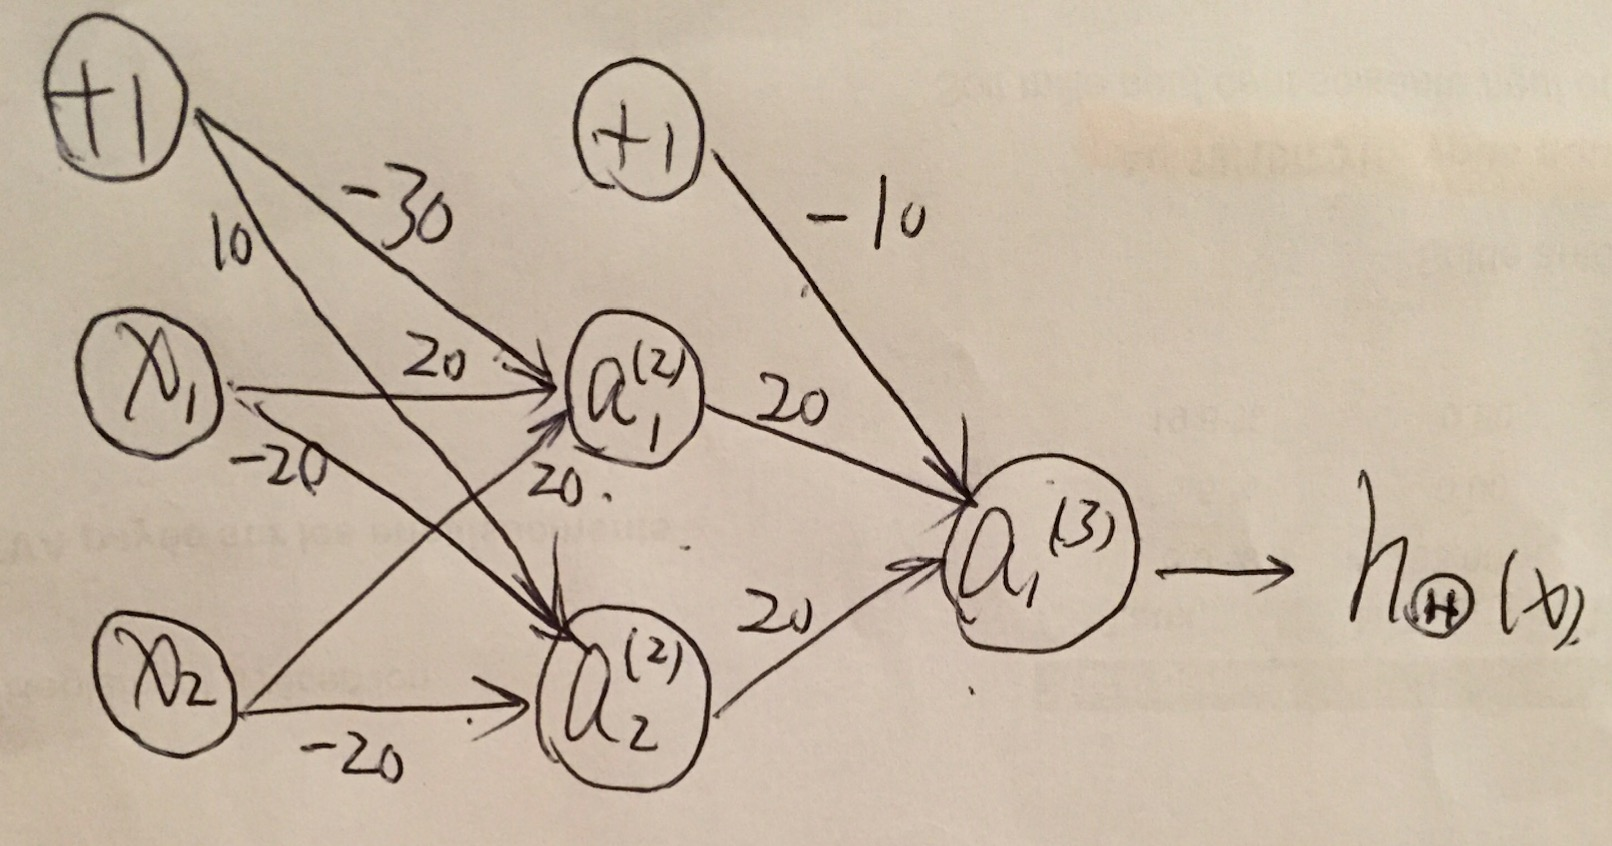
\includegraphics[width = 0.8 \textwidth]{neuralxnor.jpg}
\caption{Implementation of logical XNOR with neural network}\label{neuralxnor}
\end{figure}

Here we have \begin{math}\Theta^{(1)} = \begin{bmatrix}-30 & 20 & 20\\10 & -20 & -20\end{bmatrix}\end{math}
and \begin{math}\Theta^{(2)} = \begin{bmatrix}-10 & 20 & 20\end{bmatrix}\end{math}.

\ifx\PREAMBLE\undefined
\end{document}
\fi